%!TEX root = ../../thesis.tex
\section{Operational Transformation}
\label{sync-ot}

Operational Transformation (OT) was introduced by \cite{ellis89groupware} and resulted from their work on a groupware editor called Grove. Their technique is used in many web-based collaborative editors e.g. in Google Docs and Etherpad \cite{lautamaki2012cored}. A lot of research has been done on the topic since the original paper was issued. OT bases itself on the idea of sending operations on documents to a central server, which in turn propagates operations to all other peers. An operation is defined as a tuple of fine-grained changes to a document which contains information about the intention of the change (e.g. delete, insert), the position of where to apply the change in the document and a sometimes optional value for the change. Given the text ``HTW'', the operations \emph{O\textsubscript{1}=insert[0, ``F'']} and \emph{O\textsubscript{2}=delete[1, 1]} will result in the new text ``FTW''.

Each client in the network begins with the same document and from then will only send and receive operations on that document, updating the original itself. In that way, the network traffic is kept to a minimum and the server work is reduced because clients merge operations themselves. However, this architecture and the latency of the transport medium (nowadays the Internet) cause problems when operations overlap:

\begin{figure}[htb]
  \centerline{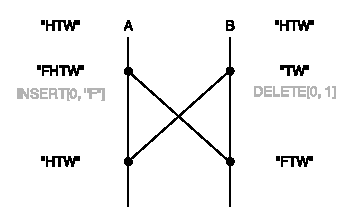
\includegraphics[width=0.8\linewidth]{images/Operational_Transformation.pdf}}
  \caption[Overlapping Operations in OT - based upon
  \protect\newline{\small\cite{nichols95jupiter}}]{Overlapping Operations in OT}
  \label{fig:OT}
\end{figure}

Client A and Client B both insert a character into the document at the same position, at the same time. The resulting text for Client A is now ``FHTW'' and the text for Client B is ``TW''. Both changes are sent to the other peers (a communication server is left out in the diagram) where they are applied to the local documents. When Client A applies the operation to the document it generates ``HTW'', but when Client B applies it to the document, the resulting text is ``FTW'' meaning that both documents diverge and the intentions of the original operations are not preserved.

A proposed solution from the original paper is to delay the execution of operations until they are executed in the correct order and, if the operations contain overlapping changes, to transform the operations in a way so that they preserve the original intention (dOPT\footnote{\cite[p. 403f]{ellis89groupware}}). The solution in its original form was limited however to P2P connections, divergence of just one step and was proven to be incorrect by \cite{cormack1995counterexample}. 

Another solution for a ``concurrency control'' system was described by \cite{nichols95jupiter} and is derived from their work on a multi-user multimedia collaboration tool named Jupiter. Instead of allowing peers to exchange their operations directly, their approach is to put a synchronization server in between, thus taking care of broadcasting the changes to all clients. In their algorithm, the transformation of operations is handled on the client and the server. When clients receive an operation that conflicts with their own last operation, they create a transformed operation from a \code{transform()} method for which the following needs to apply: $C' * S = S' * C$, where $C$ is a client operation, $C'$ a transformed client operation, $S$ a server operation and $S'$ a transformed server operation \cite[6:30min]{whitelaw2009ot}. Fundamentally this means, that client and server are capable of reaching identical documents by resolving operation conflicts on their own sides and therefore \textbf{Convergence} is guaranteed.

Since the release of the original research papers, there have been a number of papers introducing new algorithms that improve OT's characteristics and lead to more stable systems that also comply with \textbf{intention preservation} and \textbf{causality preservation} e.g. \cite{sun1998achieving} and \cite{wang2010wave}. 
Yet, most OT implementations are based on a combination of many different algorithms, chosen dependent on the system's requirements. This makes the implementation of an OT system both non-trivial and time-consuming, a common critique of OT \cite{gentle2011sharejs}.

By design, OT fulfills all User Experience requirements because it allows clients to edit the document locally (\textbf{Latency Hiding}), yet does not lock the document or parts of the document (\textbf{Full Concurrency}) and has the capability of detecting and handling diverging documents (\textbf{Graceful Exit}).